\chapter{Analysis}

This section analyses the initial problem described in the introduction. The analysis methods used originates from \cite{mathiassen2001objektorienteret}. 

\section{Introduction}
This chapter aims to provide insight in the system of which this project is based around. The sections and structure of the chapter originates from~\citetitle{mathiassen2001objektorienteret} and includes some of the techniques from~\citetitle{benyon2013designing}. Some general concepts in the system are sought to be derived from the state of the art and how these concepts affects the system is explored further. Based on concepts described in \cref{StateOfTheArt}, a paper prototype of a mobile application is presented in \cref{paperPrototypeSystemChoice}. Conclusively, a specific system definition defines the system of which this project will revolve around.

\section{Interviews}
\label{interviews}

Understanding the people involved in the system is key when doing an analysis, to find their requirements and needs of the system. It is important to get an understanding of current workflows and problems associated with these. One technique towards gaining an understanding of the users, is by interviews. The following section describes how the interviews were conducted and the results that were collected.

\subsection{Procedure}
\label{sub:procedure}
Interviews can be structured, unstructured or anything in between~\cite{benyon2013designing}. Structured interviews are very strict in their form. Every question is pre-made and the interviewer follows the questions strictly. This reduces the effort needed by the interviewer and allows the questions to be well organised and better planned. However this type of interviews should only be used when the answers given by the interviewee are simple and can fall into discrete categories.

On the other end, unstructured interviews allow for a high degree of flexibility. This form of interview is good when knowledge in a particular field is not easily accessible. This flexibility comes with the need for the interviewer to be able to generate questions on the fly and the possibility that these questions are not planned as well and possibly do not cover all aspects.

The interviews described in this section are all semi-structured i.e. most questions are written beforehand but the interviewer is not strictly bound to these and can therefore drill into particular answers given, by following up with related improvised questions. Hence the semi-structured nature of the interviews.

\subsection{Data Collection}
\label{sub:data_collection}
During the interviews the participants were voice recorded and a designated interview helper was taking notes and managing the voice recordings.

\subsection{Interview Analysis}
\label{sub:interview_analysis}
After all the interviews were performed, the group collaboratively created a summary of the interviews, in note-form, by reviewing the voice recordings. Based on the unstructured note-form summary, a more structured summary was made by categorising the notes into key topics. With the more structured interview data, the differences and similarities of the answers given by the participants are now easily extractable. The refined interview data follow each section.

\subsection{Participants}
An important choice in interviewing is who to speak with. There exists two types of people in the interaction this project works with; the bar manager or bartender, who administrates services and protects the interests of the bar, and the guests who visit the bar. The first round of interviews conducted was focused on the administers and can be found in \cref{sub:administersinterviews}. The second round was conducted with the guests at the venue and can be found in \cref{userInterviews}.

\section{Interviews with Administrators}
\label{sub:administersinterviews}
The questions for the administrators were based in the following categories:

\begin{itemize}
  \item Management of bar music systems
  \item Handling requests from the guests
  \item Current and former music systems
  \item Music requirements and the dynamics thereof
\end{itemize}

The full interview guide can be found in \cref{app:interview_guide}.

As this report focuses on the context of bars, the participants would have to have experience working at a bar and using the current music system at the bar. Therefore the sensible choice is to find participants in bars. There are different types of bars: sports bars, bars with DJs at night and bars with a pub atmosphere.

It was chosen to conduct interview with four bars, to get a good representative view of most bars.

\subsection{Control}
\label{sub:Control}
Bars use music to create their image, and music can often be the deciding factor when people are deciding to stay or leave. Therefore all bars expressed, that they want to be in full control of the music, and have the ability to override any request and rearrange the playlist if they feel the need to.

\subsection{Music Flow}
\label{sub:MusicFlow}

All bars want to be able to control the flow of the music. For instance, they do not want a slow track playing right after a party hit in the middle of a party night. This is currently managed by prepopulating a playlist from which the music system plays tracks. Guests can at any time request a track to be played, but no guarantees are given whether the requested track is played or not. When a request is given, the bartender must be the judge of whether or not the requested track is matching the current music theme.

\subsection{Music Systems and DJ}
\label{sub:differences}
Two of the bars have no DJ employed so their music system is in use throughout their opening hours, while the two others have a dedicated DJ playing at night. One participant uses MiB Pro\footnote{\url{http://www.beatpro.dk/mib-bag-baren}}, while the others use Spotify\footnote{\url{https://www.spotify.com/dk/}}. A remark was made that MiB Pro did not have as large a selection of tracks as could be desired.

\subsection{Concerns with stability}
\label{sub:specific_remarks}

One bar owner is concerned with streaming music from the internet, because of potential internet failures. A backup solution working offline would be ideal.

\subsection{Summary}
\label{sub:summary}

From these interviews, requirements have been gathered based on the participants' responses. These requirements are listed beneath using the MoSCoW method introduced in~\cite{benyon2013designing}. This method provides a structured way of prioritising user requirements. It is important to prioritise all requirements because projects do not have unlimited resources, and because of this have to solve the greatest requirements first.

\subsubsection{Must have}

\begin{itemize}\label{musthave}
        \item Ability for the bar to control what music is being played
        \item The system should always play music, no disruption in playback unless desired
\end{itemize}

\subsubsection{Should have}

\begin{itemize}
        \item Ensured continuity in the tracks that are played
\end{itemize}

\subsubsection{Could have}

\begin{itemize}
        \item The ability to take music flow into account
\end{itemize}

\subsubsection{Want to have}

\begin{itemize}
        \item System works offline
\end{itemize}

\section{State of the Art}
\subsection{SecretDJ}
SecretDJ gives its users the ability to see which venues use the SecretDJ system, and which are nearest to the user. The users can add songs to the venue's playlist and give likes, via Facebook, to the songs, moving them up the playlist.\\

A new user can add four songs to a venue's playlist each day. If a user gets a lot of likes for the songs he has added to a venue's playlist, the user can rise in rank for that venue, which means the user can add more songs to that venue's playlist and that his choices are moved further up the playlist by default. 
If a user gets enough likes and is active enough, the user can rise to the rank of DJ for a venue, meaning that the user's choice of songs will always be next in line, and there is no limit to the amount of songs the user can add to the playlist.

\section{Stakeholders}
\label{interviews}

Understanding the people involved in the system is key when doing an analysis, to find their requirements and needs of the system. It is important to get an understanding of current workflows and problems associated with these. One technique towards gaining an understanding of the users, is by interviews. The following section describes how the interviews were conducted and the results that were collected.

\subsection{Procedure}
\label{sub:procedure}
Interviews can be structured, unstructured or anything in between~\cite{benyon2013designing}. Structured interviews are very strict in their form. Every question is pre-made and the interviewer follows the questions strictly. This reduces the effort needed by the interviewer and allows the questions to be well organised and better planned. However this type of interviews should only be used when the answers given by the interviewee are simple and can fall into discrete categories.

On the other end, unstructured interviews allow for a high degree of flexibility. This form of interview is good when knowledge in a particular field is not easily accessible. This flexibility comes with the need for the interviewer to be able to generate questions on the fly and the possibility that these questions are not planned as well and possibly do not cover all aspects.

The interviews described in this section are all semi-structured i.e. most questions are written beforehand but the interviewer is not strictly bound to these and can therefore drill into particular answers given, by following up with related improvised questions. Hence the semi-structured nature of the interviews.

\subsection{Data Collection}
\label{sub:data_collection}
During the interviews the participants were voice recorded and a designated interview helper was taking notes and managing the voice recordings.

\subsection{Interview Analysis}
\label{sub:interview_analysis}
After all the interviews were performed, the group collaboratively created a summary of the interviews, in note-form, by reviewing the voice recordings. Based on the unstructured note-form summary, a more structured summary was made by categorising the notes into key topics. With the more structured interview data, the differences and similarities of the answers given by the participants are now easily extractable. The refined interview data follow each section.

\subsection{Participants}
An important choice in interviewing is who to speak with. There exists two types of people in the interaction this project works with; the bar manager or bartender, who administrates services and protects the interests of the bar, and the guests who visit the bar. The first round of interviews conducted was focused on the administers and can be found in \cref{sub:administersinterviews}. The second round was conducted with the guests at the venue and can be found in \cref{userInterviews}.

\section{Interviews with Administrators}
\label{sub:administersinterviews}
The questions for the administrators were based in the following categories:

\begin{itemize}
  \item Management of bar music systems
  \item Handling requests from the guests
  \item Current and former music systems
  \item Music requirements and the dynamics thereof
\end{itemize}

The full interview guide can be found in \cref{app:interview_guide}.

As this report focuses on the context of bars, the participants would have to have experience working at a bar and using the current music system at the bar. Therefore the sensible choice is to find participants in bars. There are different types of bars: sports bars, bars with DJs at night and bars with a pub atmosphere.

It was chosen to conduct interview with four bars, to get a good representative view of most bars.

\subsection{Control}
\label{sub:Control}
Bars use music to create their image, and music can often be the deciding factor when people are deciding to stay or leave. Therefore all bars expressed, that they want to be in full control of the music, and have the ability to override any request and rearrange the playlist if they feel the need to.

\subsection{Music Flow}
\label{sub:MusicFlow}

All bars want to be able to control the flow of the music. For instance, they do not want a slow track playing right after a party hit in the middle of a party night. This is currently managed by prepopulating a playlist from which the music system plays tracks. Guests can at any time request a track to be played, but no guarantees are given whether the requested track is played or not. When a request is given, the bartender must be the judge of whether or not the requested track is matching the current music theme.

\subsection{Music Systems and DJ}
\label{sub:differences}
Two of the bars have no DJ employed so their music system is in use throughout their opening hours, while the two others have a dedicated DJ playing at night. One participant uses MiB Pro\footnote{\url{http://www.beatpro.dk/mib-bag-baren}}, while the others use Spotify\footnote{\url{https://www.spotify.com/dk/}}. A remark was made that MiB Pro did not have as large a selection of tracks as could be desired.

\subsection{Concerns with stability}
\label{sub:specific_remarks}

One bar owner is concerned with streaming music from the internet, because of potential internet failures. A backup solution working offline would be ideal.

\subsection{Summary}
\label{sub:summary}

From these interviews, requirements have been gathered based on the participants' responses. These requirements are listed beneath using the MoSCoW method introduced in~\cite{benyon2013designing}. This method provides a structured way of prioritising user requirements. It is important to prioritise all requirements because projects do not have unlimited resources, and because of this have to solve the greatest requirements first.

\subsubsection{Must have}

\begin{itemize}\label{musthave}
        \item Ability for the bar to control what music is being played
        \item The system should always play music, no disruption in playback unless desired
\end{itemize}

\subsubsection{Should have}

\begin{itemize}
        \item Ensured continuity in the tracks that are played
\end{itemize}

\subsubsection{Could have}

\begin{itemize}
        \item The ability to take music flow into account
\end{itemize}

\subsubsection{Want to have}

\begin{itemize}
        \item System works offline
\end{itemize}

\input{Chapters/Analysis/Stakeholders/personas.tex}
\section{Problem and Application Domain}
\sinote{Dette afsnit er design orienteret. Er ikke færdigt}

\textbf{Problem domain}: \enquote{That part of a context that is administrated, monitored or controlled by a system.}

\begin{description}
  \item[Tracks] The tracks that are available for playing.
  % \item[Playlists] Collections of tracks centered around a specific theme.
  \item[Votes] Some mechanism for choosing which tracks to play next.
  \item[Users] Data and statistics of the users of the system.
  \item[Places] What is playing at particular places?
  \item[Audio system] Plays the chosen track.
  \item[Display system] Displays queue, current track, etc. at the installation site.
\end{description}

\textbf{Application domain}: \enquote{The organization that administrates, monitors, or controls a problem domain.}

\begin{description}
  \item[Users] The users of the application chooses which tracks to play next.
  \item[Frontend] Provides control of tracks, playlists and users.
  \item[Backend] Administrates and monitors users of the application. Communicate with the audio- and display system.
\end{description}

\section{PACT designing for people}
%!TEX root = ../../Master.tex
When designing an interactive system it is important to think about the people using it. The people are a part of the interactive system and therefore it is important to make sure that the design fits the people. In~\cite{benyon2013designing} PACT analysis is presented as a framework for thinking about design situations. To help with the design being human centred, the designer needs to understand the four parts of the analysis: It is important to understand the different kind of people using the system, since they have different prerequisites for using a system. The activities that people want to undertake are equally important, as it says a lot about the way the system will be used. The designer needs to think about the context, the location and organisation, the system will be used in, which provide information about how the system should operate. Lastly the designer should consider the features of interactive technologies and how to incorporate them in the design.

\begin{figure}
  \centering
  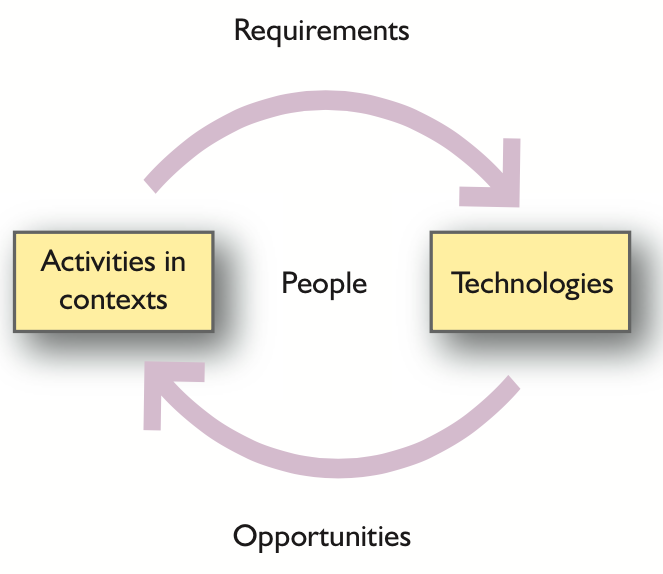
\includegraphics[width=0.5\linewidth]{pact-overview.png}
  \caption{The relationships between activities, contexts, people and technologies in PACT. From~\cite{benyon2013designing}}
  \label{fig:pact-overview}
\end{figure}

It is also important to understand the relationship between activities and technologies. \Cref{fig:pact-overview} shows how the activities people are doing will influence the requirements for technologies. This will create new technology that will change the activities people will be doing with the technology.

It is the variety of requirements that is found during the PACT analysis, that can make designing systems difficult. Therefore, an analysis of the four core elements of PACT will be conducted.


\subsection{People}
\label{sub:pact_people}

The system is used by people who go to bar-like environments, and are possibly intoxicated. At bar-like environments, music is central to the atmosphere, and a lot of people are interested in having their music tastes accommodated. Different people exhibit different behaviour in these social contexts, some may clique together when using a social system and some may be afraid of stigmas when using it. To use the system, a smartphone is required, and some people may be unable or afraid \chnote{uddyb hvorfor} to use their smartphone.

\subsection{Activities}
\label{sub:pact_activities}

Usage of the system requires the user to interact with their smartphone or similar device. Firstly the user must install the application on their device. The installation process should not take a long time, or else the user might forget about the application. When the user is checked-in, the current playlist of the venue will be displayed. The transition from the check-in to the playlist screen should occur in less than 100 milliseconds as to not frustrate the user. From the playlist screen the user can vote on a track. Finding which track to vote for should not be a complex action, as this is an expected frequently done action.

\paragraph{New or improved activities}
The system introduces a possibility of requesting a track to be played at the venue, without having to ask the administrator. This eases work load on administrator, which might be busy serving beverages to a customer. It also eases the process of requesting a track by not having to get up if sitting and splitting from one's group or partner, which may lead to a more time spend together. The system might change the behavior of the users and serve as topic of discussion, possibly an icebreaker. These changes in activities should be considered when designing the system.

\subsection{Context}
\label{sub:pact_context}

This system can be used at places where many people wants to listen to music, but does not have an efficient method \chnote{påstand, uddyb} of determining which tracks to listen to.

A dark environment with a lot of noise is common in bars/pubs. As people are often dancing in this environment, active use of smartphones is not recommended\chnote{why}. Also, usage of smartphones in these kind of environments often cause anti-social behaviour. \chnote{kilde ville være super nice :)}

\subsection{Technologies}
\label{sub:pact_technologies}

The system runs on a host computer with an audio system connected and a business license for Spotify. \chnote{meget specific?} This host computer is located at the installation site.

For users to operate this system a smartphone with internet connection and adequate battery life is required. \chnote{ved vi alle de ting? hvis det skal ikke skal være i retrospekt}
When designing the system, different smartphones and their characteristics have to be considered.

\subsection{Summary}
\label{sec:pact_summary}

As the people using the system are possibly intoxicated and in contexts of meeting and talking to other people, by speech, it is considered rude and anti-social to neglect the interactive to using a smartphone. Other ways of interacting with the system could be considered, or to minimize the time spend on smartphone usage. Therefore the system must be \textbf{quick}* \footnote{Frequent and determined users might access the system often with a already known task for the system, making them capable of communicating a request of system very quickly, the system should sought to not be the limiting factor in this process.} and \textbf{easy to navigate and use}, by focusing on providing a small and effective set of functionalities. Pervasive computing is a significant part of the system, and therefore battery saving on these mobile device is of concern, therefore a requirement of the system is to \textbf{minimize power consumption} as result of usage of the system, by not doing extensive computing on the clients side.

Also in the context of the system, the users might be dancing... \chnote{maybe relevant}

The PACT analysis provide us with these requirement:
\begin{itemize}
  \item Should be quicker than the user
  \item Easy to use and navigate - Few but effective functionalities
  \item No extensive computations on the client
\end{itemize}

\section{Architecture}
\label{sec:architecture}

This section describes how the different components of the system are
composed to build a coherent piece. A complete diagram of the
architecture can be seen in \cref{fig:architecture}.

The system is separated in two main parts: a client and a server. The
client is simpler than the server; it's main task is to display
information given by the server, and can therefore be seen as a dumb
client. All the business logic is therefore contained on the
server. This communication occurs through the System Interface
components of the client and server. This information sent back and
forth between the client and server is displayed in the User Interface
component of the client and the server.

The aforementioned business logic on the server is a collection of
many different components. Each of these components have a distinct
responsibility. For example, the UserService has the responsibility to
handle all actions related to users of the application. The
UserService component defines the functions available on users. It is
therefore placed in the function layer of the server. To perform it's
actions, the UserService component has associations to the User
component defined in the model layer of the server.

Another yet unexplained layer of the server architecture is the
technical platform. Components contained in this layer are all
libraries defined outside of the business logic of the server, but are
still required in order to provide a complete system. For example, the
SpotifyDotNet component is a library for streaming tracks from
Spotify. The implementation of this library is described in
\cref{imp:libspotify}.

\begin{figure}
  \centering
  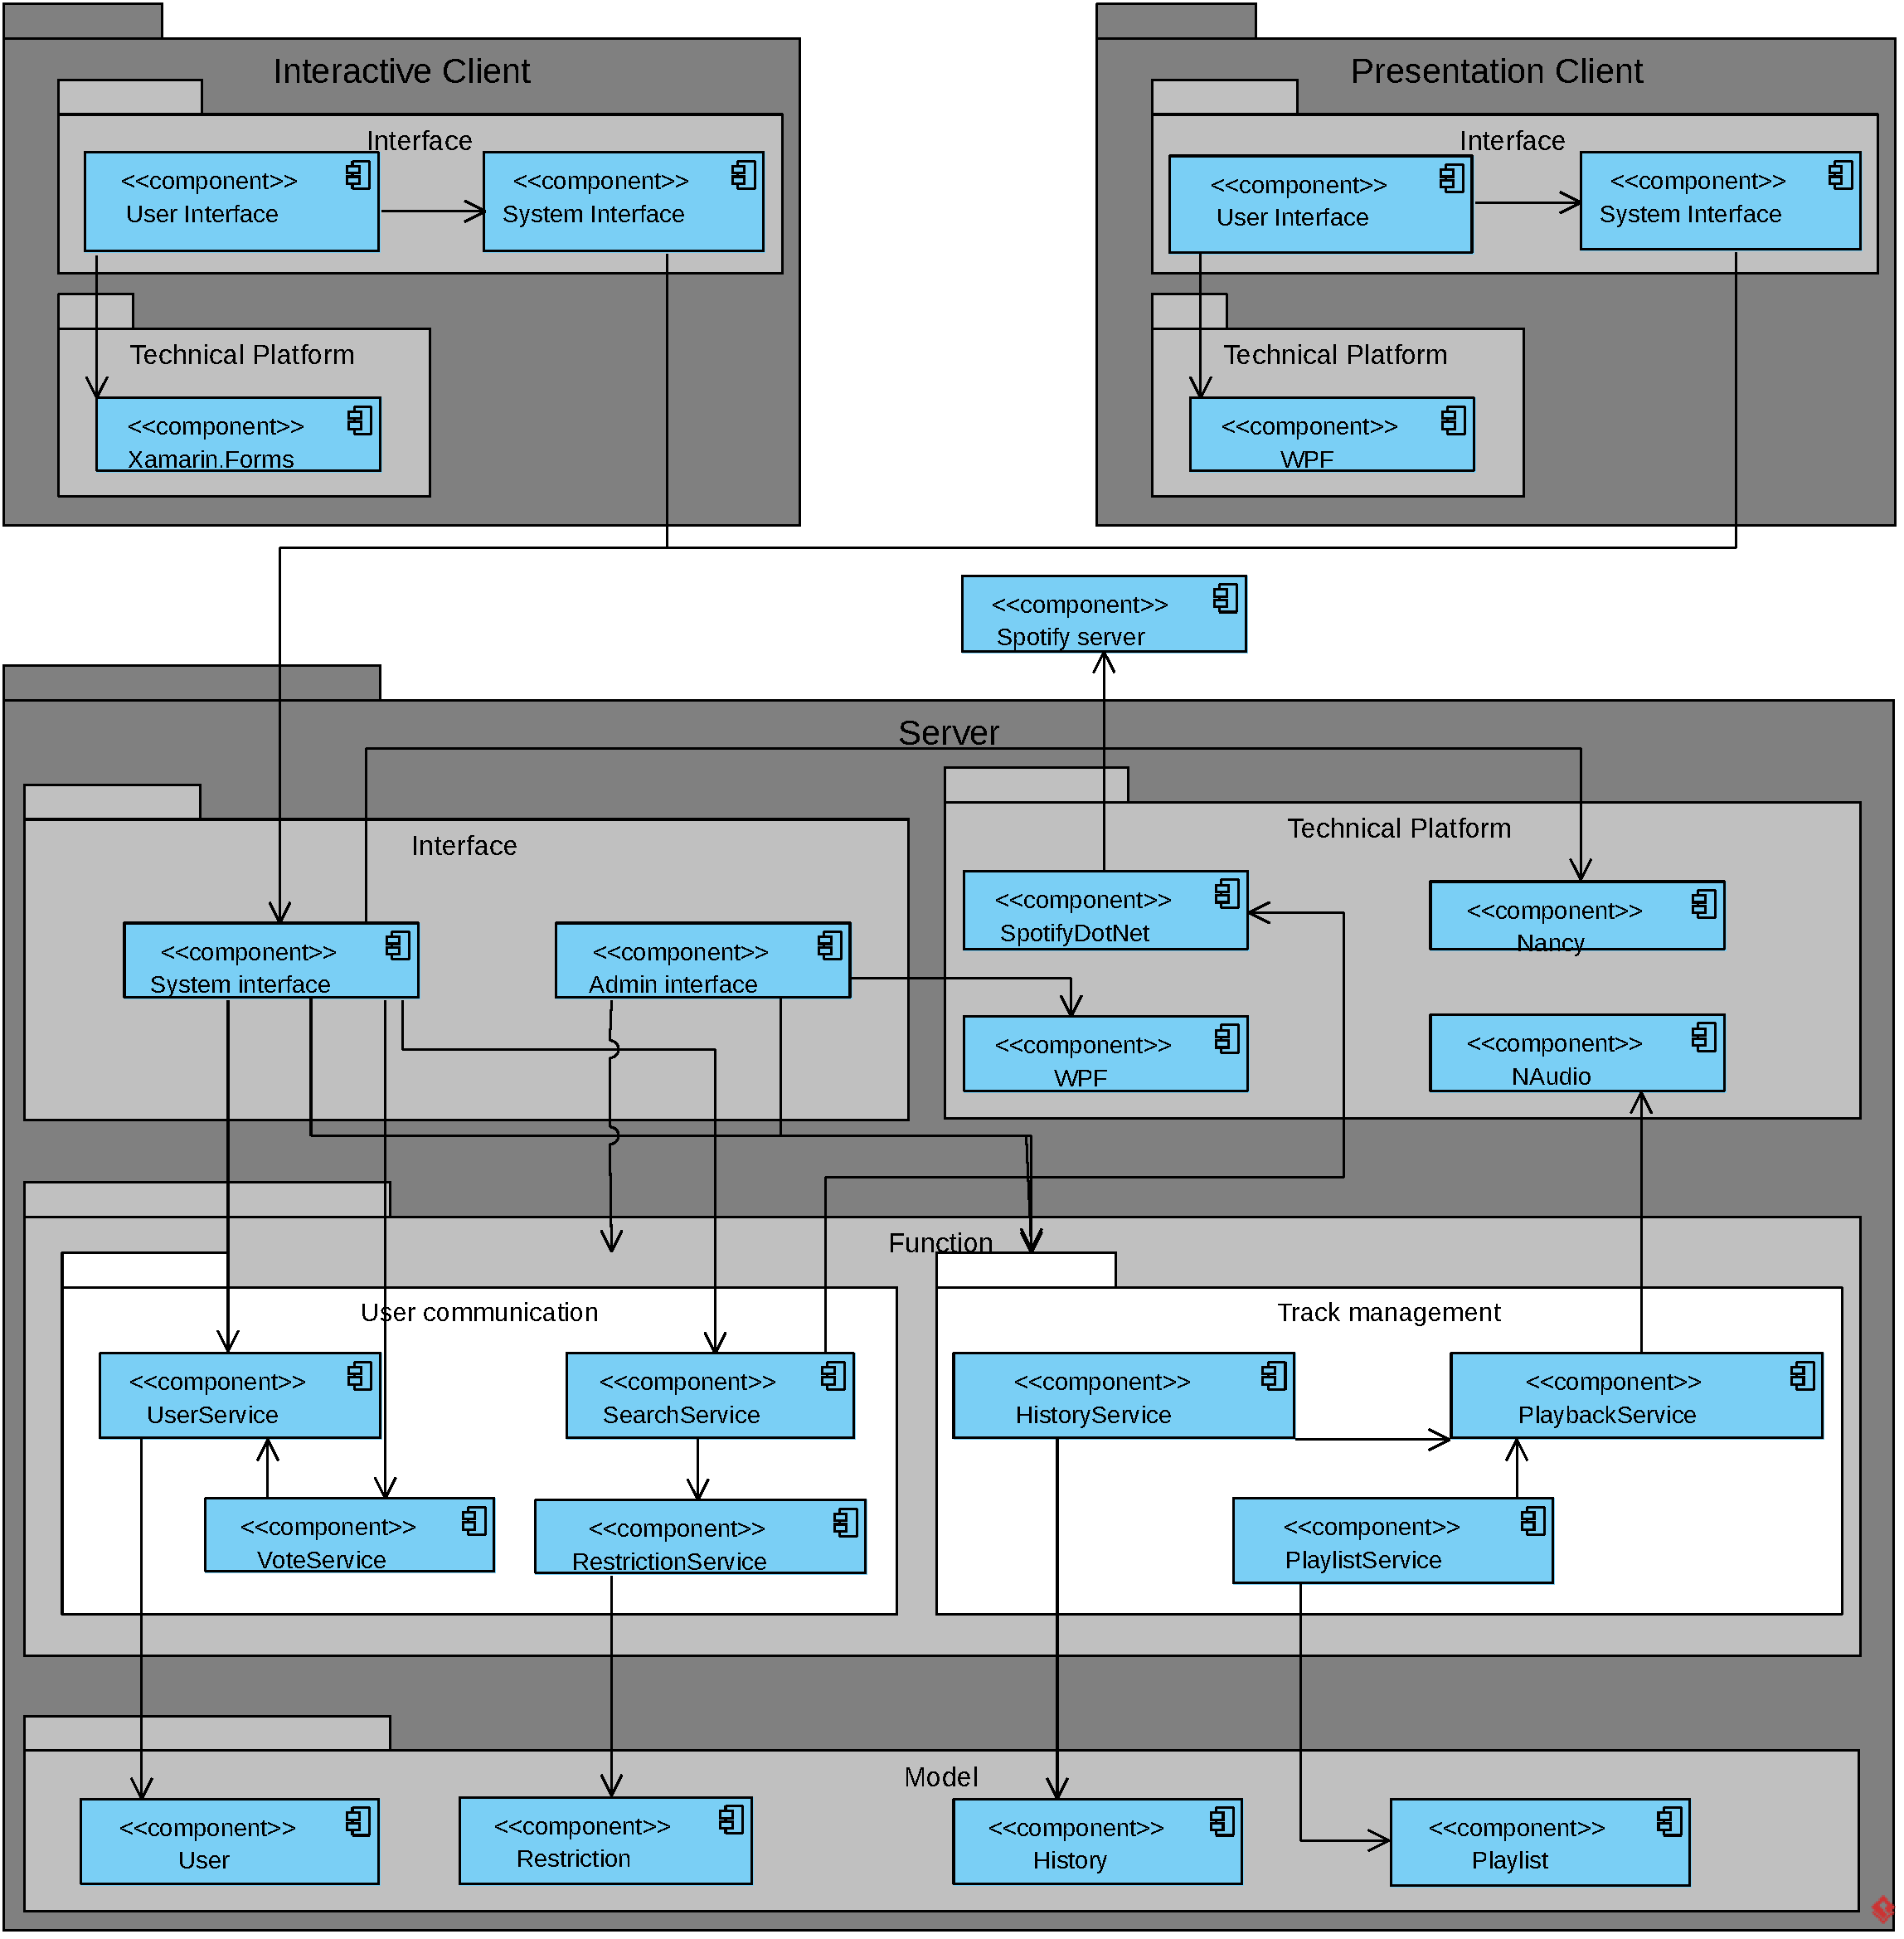
\includegraphics[width=1.2\linewidth]{Images/Arkitektur.pdf}
  \caption{Architecture of the system}\label{fig:architecture}
\end{figure}

\section{Problem Statement}
\begin{center}
\textit{How is it possible to develop a software solution which provides a venue with the ability to fairly and dynamically cater to their guests' music preferences?}
\end{center}

Furthermore, the system should take some subproblems into account:
\begin{itemize}
\item How can the system provide supervision and control to the administrators?
\item How can the system avoid undesirable music flow?
\end{itemize}
